\documentclass[../Kvantemekanik.tex]{subfiles}
 
\begin{document}


\section{Den uendelige potentialebrønd}
Den første udgave af Schrödingerligningen vi skal løse, er en ægte klassiker, nemlig den uendelige potentialebrønd. Dette er nok det potentiale, der er nemmest at løse for Schrödingerligningen, og løsningen til dette potentiale benyttes faktisk en del steder i fysikken, da mange lukkede systemer kan approksimeres til at være uendelige potentialbrønde i 1, 2 eller 3 dimensioner, alt efter hvordan systemet er indrettet.

I den uendelige potentialebrønd forestiller vi os, at partiklen er fanget i et potentiale, der er $V(x)=0$ for $0<x<L$ inde i brønden, og uden for brønden er potentialet uendelig stort, $V(x)=\infty$ for $x<0$ og $x>L$. Når man begynder at arbejde med uendeligheder bliver ens resultater ofte lidt funky, for hvordan skal man fysisk tolke noget, der er uendelig stort?

I dette tilfælde vil det betyde, at partiklen skal have uendelig meget energi for at være i området uden for brønden, og da det selvfølgelig ikke giver nogen fysisk mening at have en partikel med uendelig meget energi, betyder det, at sandsynligheden for at finde partiklen udenfor brønden, må være uendelig lille, eller sagt med andre ord lig med nul (dette er en af de eneste potentialer, hvor man definitivt kan sige at sandsynligheden for at finde en partikel et bestemt sted er lig med nul).
\begin{figure}[h]
    \centering
    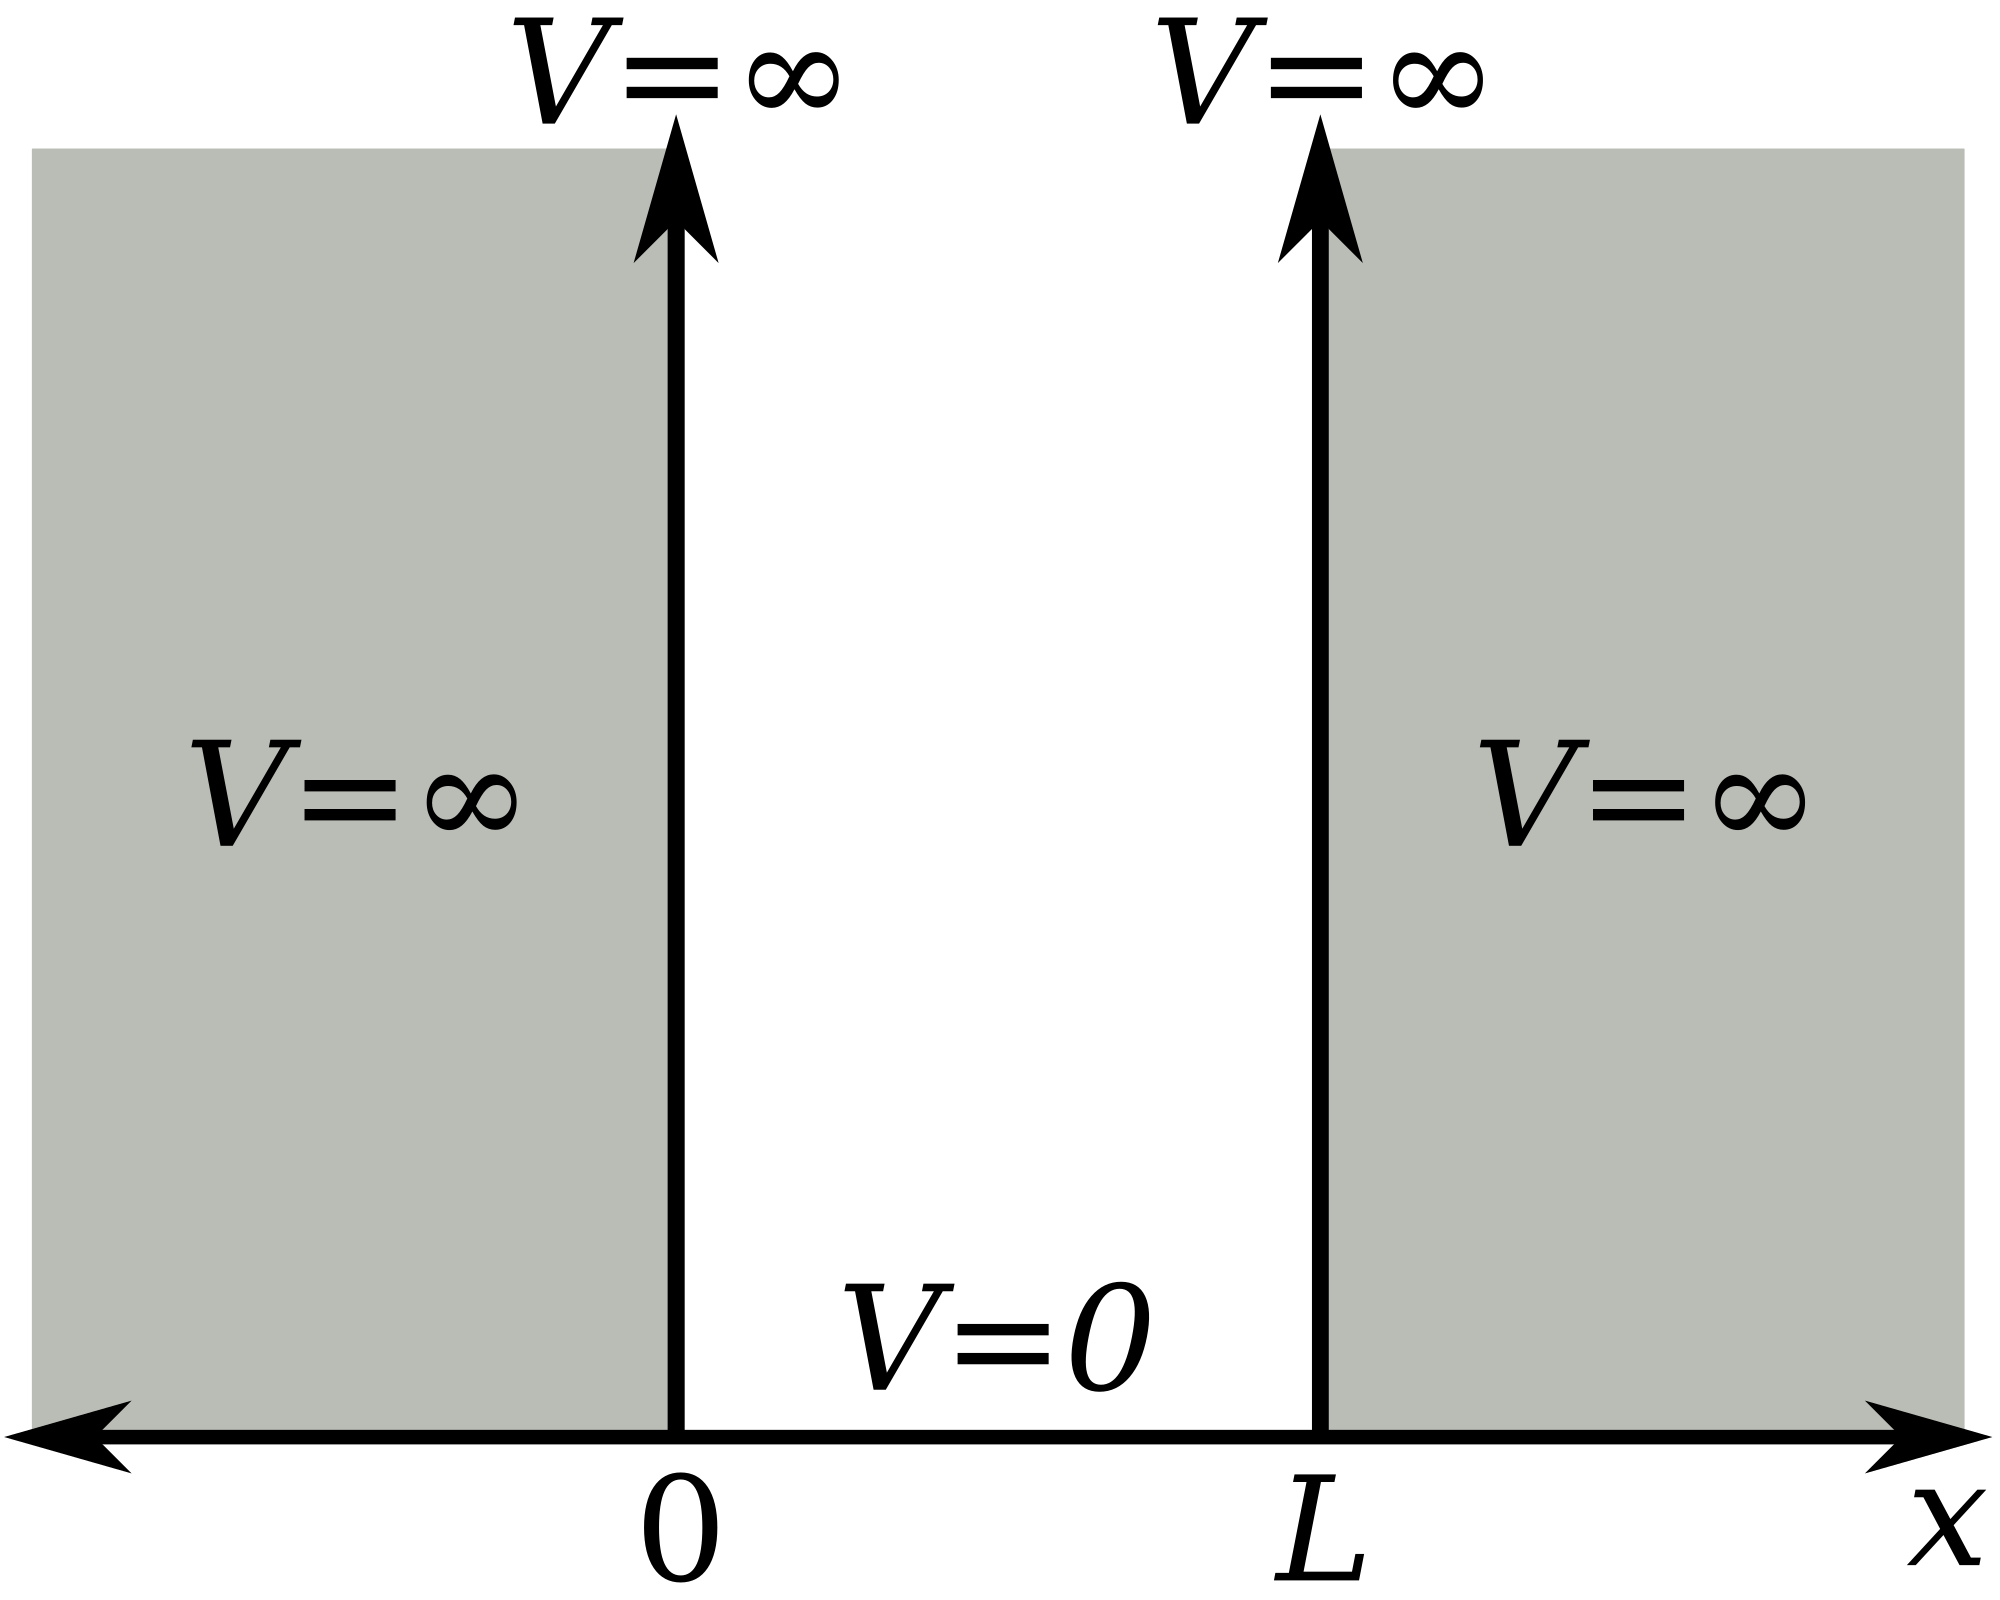
\includegraphics[scale=0.13]{Kvantemekanik/billeder/uendelig.png}
    \caption{Skitse af den uendelige potentialebrønd}
    \label{fig:uendelig}
\end{figure}

For at finde løsningen til Schrödingerligningen, behøver vi kun at koncentrere os om området inde i brønden, da dette er det eneste sted partiklen kan være. På grund af potentialet kræver vi samtidig, at bølgefunktionen må være nul ved $x=0$ og $x=L$, dette leder til at Schrödingerligningen tager formen:
\begin{equation}
    \frac{-\hbar^2}{2m}\pdif[2]{x}\psi=E\psi
    \label{kvant:eq:infb}
\end{equation}
Bølgefunktionerne er altid kontinuerte. Så siden bølgefunktionen er nul alle steder uden for brønden, må den også være det ved kanten af brønden:
$$
\psi(0)=\psi(L) = 0
$$
Omskrives den tidsuafhængige Schrödingerligning lidt, finder vi differentialligningen:
\begin{equation}
\pdif[2]{x}\psi = \frac{-2mE}{\hbar^2}\psi = -\left(\frac{\sqrt{2mE}}{\hbar}\right)^2\psi = -k^2\psi
\end{equation}
Her indføres $\omega = \frac{\hbar}{\sqrt{2mE}}$, for at gøre de følgende udregninger markant pænere.
Da $\dif[2]{x}{}\cos(x) = -\cos(x)$ og $\dif[2]{x}{}\sin(x) = -\sin(x)$, er det oplagt at løsningerne til Schrödingerligningen er baseret på trigonometriske funktioner. Ganske rigtigt er den generelle løsning til differentialligningen på formen:\footnote{Tjek at det passer.}
\begin{equation}
\psi = A\sin k x+B\cos k x
\end{equation}
Konstanterne $A$, $B$ og $k$ (og dermed $E$), kan ikke være hvad som helst. Deres værdier skal passe med grænsebetingelserne. Lad os til at starte med betragte $L=0$. Her er bølgefunktionen:
\begin{equation}
\psi(0) = A\sin(0)+B\cos(0) = B = 0
\end{equation}
Vi kan hermed konkludere at $B=0$. Bølgefunktionen er dermed en sinusfunktion.
Den anden ende af brønden giver os værdien af $k$, og dermed $E$. 
\begin{align*}
&\psi(L) = A\sin(k L) = 0\\
\implies &\sin(k L) = 0\\
\implies &k L = \pi n
\end{align*}
Her kan $n$ være et hvilket som helst helt tal større end eller lig 1. Der er altså mere end en mulig værdi for $k$, og de forskellige værdier er klart forskellige. Vi har netop fundet at $k$ og dermed også energien er kvantiseret. De kan have værdierne:
\begin{align}
k_n &= \frac{\pi n}{L}\\
E_n &= \frac{k^2\hbar^2}{2m} = \frac{\pi^2n^2\hbar^2}{2mL^2}
\end{align}
Nu mangler blot at finde konstanten $A_n$ for alle $n$. Den kan findes ud fra normeringskravet, der følger af sandsynlighedsfortolkningen af bølgefunktionen.
$$
\braket{\psi}{\psi} = \integral{\abs{\psi}^2}{x}{-\infty}{\infty} = 1
$$ 
Siden bølgefunktionen er nul alle andre steder end i brønden, vil integralet også være det. Derfor skal der kun integreres her
$$
\braket{\psi}{\psi} = A^2\integral{\sin^2(\tfrac{\pi n x}{L})}{x}{0}{L} 
$$
Der er rigtigt mange regneregler for trigonometriske funktioner, men en af dem der ofte er nyttig er: $\sin^2(x) =\frac{1}{2}-\frac{1}{2}\cos(2x)$. Bruges den bliver integralet:
$$
\braket{\psi}{\psi} = \frac{A^2}{2}\integral{\big(1-\cos(\tfrac{2\pi n x}{L})\big)}{x}{0}{L} = \frac{A^2L}{2}-\frac{L}{2\pi n}\left[\sin(\tfrac{2\pi nx}{L})\right]_0^L = \frac{A^2L}{2}-\frac{L}{2\pi n}+\frac{L}{2\pi n} = \frac{A^2L}{2} = 1
$$
Det er nu muligt at isolere $A$.
\begin{equation}
A=\sqrt{\frac{2}{L}}
\end{equation}
Nu kan det konkluderes, at de stationære løsninger til den uendelige brønd er:
\begin{equation}
\psi_n(x) = \sqrt{\frac{2}{L}}\sin\left(\frac{\pi nx}{L}\right)~~~~~~n\in \N\backslash\{0\}
\end{equation}
\begin{figure}
\center
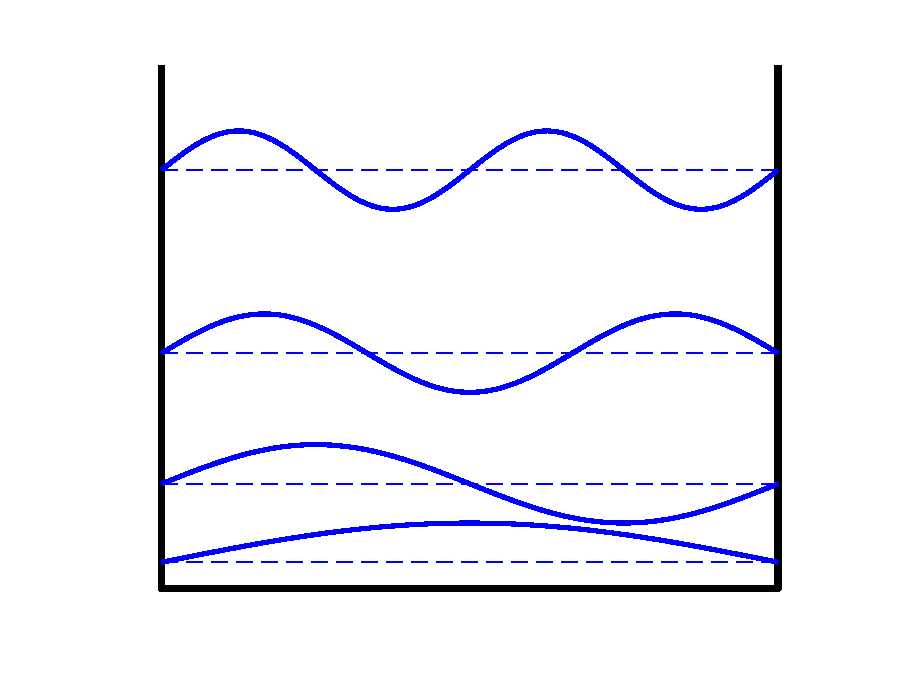
\includegraphics[width = 0.75 \textwidth]{Kvantemekanik/billeder/infwellwave.eps}
\caption{De laveste fire bølgefunktioner for den uendelige brønd forskudt efter deres energi.}
\end{figure}


\end{document}